\section*{Problem 4}

Repeat Problem 3 for $x(t) = 2 + \cos(50 \pi t)$ and T = 0.025 sec.

\begin{itemize}
\item  Draw $|X_s(\omega)|$ where $x_s(t) = x(t)p(t)$. Determine if aliasing occurs.
\end{itemize} 

\subsection*{Solution}

Since $T_s = 0.025 sec$ is greater than the minimum required,
aliasing will occur as can be seen in (\ref{fig:c3p4a}).

\begin{equation*}
\omega_s = \frac{2 \pi}{T_s} =  80 \pi
\end{equation*} 

\begin{figure}[H]
\caption{Sampling $|X_s(\omega)|$}
\centering
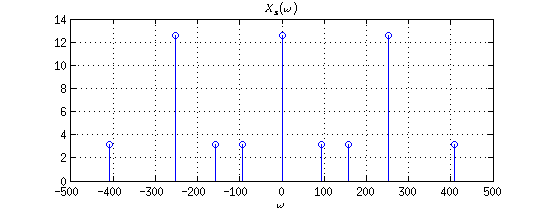
\includegraphics[width=0.8\textwidth]{figs/c3p4a.png}
\label{fig:c3p4a}
\end{figure}

\begin{itemize}
\item Determine the expression for y(t).
\end{itemize} 

\subsection*{Solution}

The limits of the lowpass filter are $-0.5 \omega_s = -40 \pi$ to $0.5 \omega_s = 40 \pi$.
The Fourier transform of $Y(\omega) = H(\omega)X(\omega)$ is:

\begin{figure}[H]
\caption{Magnitude $|X(\omega)|$}
\centering
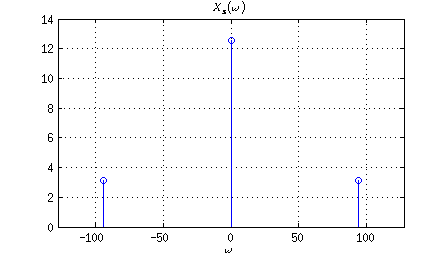
\includegraphics[width=0.6\textwidth]{figs/c3p4b.png}
\label{fig:c3p4b}
\end{figure}

And therefore:

\begin{equation*}
\begin{aligned}
y(t) = 2 + \cos(30 \pi t)
\end{aligned}
\end{equation*} 

\begin{itemize}
\item Determine an expression for x[n].
\end{itemize} 

\subsection*{Solution}

\begin{equation*}
\begin{aligned}
x(n) &= 2 + \cos(50 \pi n T_s) \\
     &= 2 + \cos(1.25 \pi n)
\end{aligned}
\end{equation*} 
